\documentclass[12pt]{article}
\usepackage{amsmath, amssymb, amsthm}
\usepackage[margin=1in]{geometry}
\usepackage{fancyhdr, enumitem}
\usepackage{graphicx, tikz}
\usepackage[labelfont=bf]{caption}

\pagestyle{fancy}
\fancyhf{}
\chead{PROBLEM SET 2}
\rhead{Elliot Ahn}
\lhead{Machine Learning}
\rfoot{\thepage}

\setlength{\headheight}{15pt}
\renewcommand{\footrulewidth}{0.5pt}

\begin{document}
\begin{enumerate}[leftmargin=*]
\item (b) See python figures
\item (d) $c_{\text{min}}$ is the only one where the samples are not independent.
\item (e)
\begin{align*}
P \left( y = f(x) \neq h(x) \right) &= \lambda \mu \\
P \left( y \neq f(x) = h(x) \right) &= (1 - \lambda) (1 - \mu)
\end{align*}
So
\[ P \left( y \neq h(x) \right) = \lambda \mu + (1 - \lambda) (1 - \mu) \]
\item (b) Collect all $\mu$ terms and set the coefficient to zero.
\[ \lambda \mu + 1 + \lambda \mu - \lambda - \mu \]
\[ (2 \lambda - 1) \mu = 0 \implies \lambda = \frac{1}{2} \]
\item (c)
\item (c)
\item (a)
\item (d) This also follows from symmetry since averaging out the linear regressio weights implies that the line goes through the middle of the sample space implying that half the points are on the wrong side.
\item (a)
\begin{center}
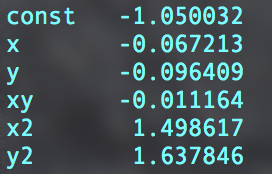
\includegraphics[scale=1]{NonLinearReg}
\end{center}
\item (b)
\end{enumerate}
\end{document}